\section{WiFi-Adapter testen}
Es lohnt sich, zuerst überprüfen, ob der angeschaffte WiFi-Adapter auf dem aufgespielten Betriebssystem lauffähig ist. Dazu muss man lediglich den Adapter in den USB-Port stecken und nach kurzer Wartezeit folgendes Kommando aufrufen:

\begin{lstlisting}
ifconfig -a
\end{lstlisting}

Wenn auf der erschienen Ausgabe einen Eintrag für \textit{wlan0} zu sehen ist, kann mit der Einrichtung des Access Points begonnen werden.

% FIXME: Was, wenn wlan0 nicht auftaucht?
% FIXME: Bild von ifconfig?
% FIXME: Bild von Pi mit eingesteckter Antenne?

\section{Access Point einrichten}
Mit dem eingesteckten Netzwerkkabel und dem per USB angeschlossenen WiFi-Adapter stehen nun zwei Netzwerk-Schnittstellen zur Verfügung. Das Netzwerkkabel hat die Aufgabe, den Raspberry Pi mit dem Internet zu verbinden. Der WiFi-Adapter hingegen soll so eingerichtet werden, dass er ein lokales WLAN aufzieht. Der Raspberry Pi fungiert somit als Wireless Access Point. Ein Wireless Access Point ermöglicht es Geräten wie Notebooks oder Smartphones, sich über ihn kabellos mit dem Internet zu verbinden. Neben der Software für den Access Point selbst wird ein eigener DHCP-Server benögtigt. Dieser ist dafür verantwortlich, dass jeder Computer, der sich mit dem WLAN verbindet, eine valide IP-Adresse erhält und somit ein Teil des Netzes werden kann.

Mit folgenden befehlen können die benötigten Softwarekomponenten installiert werden.
 
\begin{lstlisting}
apt-get install hostapd isc-dhcp-server
\end{lstlisting}

\subsection{DHCP-Server konfigurieren}
Damit der DHCP-Server auch richtig funktioniert, muss er zuerst konfiguriert werden.
Dazu öffnet man die Datei \textit{/etc/dhcp/dhcpd.conf} mit einem Texteditor. Hier wird dazu der vorinstallierte Texteditor Nano verwendet.

\begin{lstlisting}
nano /etc/dhcp/dhcpd.conf
\end{lstlisting}

Zuerst müssen die folgenden Zeile gefunden und mittels einer vorangestellten Raute (\#) auskommentiert werden. Auskommentiert bedeutet, dass die Zeile ungültig und somit nicht mehr aktiv ist.

\begin{lstlisting}
option domain-name "example.org"
option domain-name-server ns1.example.org,ns2.example.org
\end{lstlisting}

Neu sieht das ganze folgendermassen aus:

\begin{lstlisting}
#option domain-name "example.org"
#option domain-name-server ns1.example.org,ns2.example.org
\end{lstlisting}

Als nächstes muss dem DHCP-Server mitgeteilt werden, dass er der offizielle DHCP-Server dieses Netzes ist. Einmal eingestellt vergibt er fortan valide IP-Adressen an jeden Client, der ihn per DHCP-Request anfragt.
Dazu muss folgende Zeile einkommentiert - die vorangestellte Raute entfernt - werden.
\\
Aus

\begin{lstlisting}
#authoritative;
\end{lstlisting}

wird:

\begin{lstlisting}
authoritative;
\end{lstlisting}

Für das WLAN, das künftig vom WiFi-Adapter aufgezogen wird, müssen auch noch diverse Einstellungen festgelegt werden.
Man fügt dazu folgende Zeilen ans Ende der Datei an:

\begin{lstlisting}
subnet 192.168.66.0 netmask 255.255.255.0 {
  range 192.168.66.10 192.168.66.50;
  option broadcast-address 192.168.66.255;
  option routers 192.168.66.1;
  default-lease-time 666;
  max-lease-time 7200;
  option domain-name "local";
  option domain-name-servers 8.8.8.8, 8.8.4.4;
}
\end{lstlisting}

Den DHCP-Server ist nun fertig konfiguriert. Jetzt muss er an ein Netwerkinterface gebunden werden. Das gesuchte Netzwerkinterface ist in diesem Fall wlan0, wie man schon zu beginn mittels ``ifconfig'' herausgefunden hat.
In der Datei \textit{/etc/default/isc-dhcp-server} muss dazu bei der Einstellung \textit{INTERFACES} wlan0 eingetragen werden:

\begin{lstlisting}
INTERFACES="wlan0"
\end{lstlisting}

Dem Interface \textit{wlan0} kann jetzt eine statische IP-Adresse vergeben wird. Es handelt sich dabei um jene Adresse, die bei der Konfiguration des DHCP-Server bei \textit{option routers} angegeben wurde (192.168.66.1). \\
In der Datei \textit{/etc/network/interfaces} müssen die Zeilen:

\begin{lstlisting}
iface wlan0 inet manual
wpa-roam: /etc/etc/wpa_supplicant/wpa_supplicant.conf
iface default inet dhcp
\end{lstlisting}

Mit den folgenden ersetzt werden:

\begin{lstlisting}
iface wlan0 inet static
  address 192.168.66.1
  netmask 255.255.255.0
\end{lstlisting}

% FIXME: Bild von fertigem interfaces file?

Das Interface \textit{wlan0} läuft zu diesem Zeitpunkt bereits. Damit die Änderung sofort wirksam wird, kann man dem Interface mit folgendem Befehl die zuvor definierte IP-Adresse aufzwingen:

\begin{lstlisting}
ifconfig wlan0 192.168.66.1
\end{lstlisting}

% FIXME: ifconfig oder ifup?

\subsection{Hostapd konfigurieren}
Weiter geht es darum den Access Point selbst einzurichten. Die verwendete Software \textit{hostapd} wurde zu Beginn des Abschnitt bereits installiert. 
Wie schon beim DHCP-Server, müssen auch hier gewisse Konfigurationen vorgenommen werden. Das Konfigurationsfile für hostapd gibt es noch nicht, weshalb man zuerst eines erstellen muss:

\begin{lstlisting}
touch /etc/hostapd/hostapd.conf
\end{lstlisting}

Danach das File mit einem Texteditor öffnen:

\begin{lstlisting}
nano /etc/hostapd/hostapd.conf
\end{lstlisting}

Und folgende Zeilen hinzufügen:

\begin{lstlisting}
interface=wlan0
driver=r8712u
ssid=PiProxy
hw_mode=g
channel=6
macaddr_acl=0
auth_algs=1
ignore_broadcast_ssid=0
wpa=2
wpa_passphrase=pi
wpa_key_mgmt=WPA-PSK
wpa_pairwise=TKIP
rsn_pairwise=CCMP
\end{lstlisting}

Ein paar der obigen Werte kurz erklärt: 
\begin{itemize}
\item driver: Der Treiber des Wifi-Adapters, ist je nach Adapter anders und muss daher zuerst ausfindig gemacht werden
\item ssid: Der Name des Netzes, wie man es nach aussen hin sieht
\item wpa\_passphrase: Passwort des Netzes, sollte gut gewählt werden, um optimale Sicherheit zu bieten
\end{itemize}

% FIXME: Beschreiben, wie Treiber ausfindig gemacht werden kann?

Diese nun erstellte Konfiguration muss \textit{hostapd} bekannt gemacht werden. In der Datei \textit{/etc/default/hostapd.conf} muss nach \textit{DAEMON\_CONF} gesucht und die Zeile wie folgt verändert werden:

\begin{lstlisting}
DAEMON_CONF="/etc/hostapd/hostapd.conf"
\end{lstlisting}

Der Raspberry Pi ist nun soweit, ein WLAN aufziehen und sich mit dem Internet verbinden zu können. Was noch fehlt ist die Verbindung dazwischen.

\subsection{NAT konfigurieren}
NAT (Network Address Translation) wird verwendet, um die mit dem WLAN verbundenen Geräte ins Internet weiterzuleiten.

Zuerst wird der Datei \textit{/etc/sysctl.conf} folgendes angefügt:

\begin{lstlisting}
net.ipv4.ip_forward=1
\end{lstlisting}

Damit die Weiterleitung im laufenden Betrieb aktiviert wird, muss der folgende Befehl ausgeführt werden:

\begin{lstlisting}
echo 1 > /proc/sys/net/ipv4/ip_forward
\end{lstlisting}

Zusätzlich muss die Firewall so eingestellt werden, dass NAT das eingerichtete Forwarding ausführen kann:

\begin{lstlisting}
iptables -t nat -A POSTROUTING -o eth0 -j MASQUERADE

iptables -A FORWARD -i eth0 -o wlan0 -m state --state RELATED,ESTABLISHED -j ACCEPT

iptables -A FORWARD -i wlan0 -o eth0 -j ACCEPT
\end{lstlisting}

Damit man diese Befehle nicht bei jedem Neustart des Raspberry Pi eingeben muss, können sie permanent gespeichert werden:

\begin{lstlisting}
iptables-save > /etc/iptables.ipv4.nat

echo "up iptables-restore < /etc/iptables.ipv4.net" >> /etc/network/interfaces
\end{lstlisting}

\section{Aufstarten von hostapd und dem DHCP-Server}
Bevor der Access Point getestet werden kann, müssen alle beteiligten Komponenten gestartet werden:

\begin{lstlisting}
service hostapd start
service isc-dhcp-server start
\end{lstlisting}

% FIXME: Wie testen? Bild von Netzwerk?

\section{Tor aufsetzen}
Es ist nun möglich, sich mittels Access Point mit dem Internet zu verbinden. Das Ziel ist es aber, dass diese Verbindung ins Internet über das Tor-Netzwerk erfolgt. Tor kann man, wie die zuvor verwendeten Programme auch, über die Paketverwaltung installieren:

\begin{lstlisting}
apt-get install tor
\end{lstlisting}

Nach der Installation muss Tor natürlich noch entsprechend konfiguriert werden. Dazu öffnet man die Konfigurationsdatei mittels Texteditor: 

\begin{lstlisting}
nano /bla bla bla
\end{lstlisting} 

% FIXME: Pfad von torrc angeben

Direkt nach dem einleitenden Kommentarblock müssen folgende Zeilen hinzugefügt werden:

\begin{lstlisting}
Log notice file /var/log/tor/notices.log
VirtualAddrNetwork 10.192.0.0/10
AutomapHostsSuffixes .onion,.exit
AutomapHostsOnResolve 1
TransPort 9040
TransListenAddress 192.168.66.1
DNSPort 53
DNSListenAddress 192.168.66.1
\end{lstlisting}

Die Datei sollte nun folgendermassen aussehen: 

\begin{figure}[h]
\centering
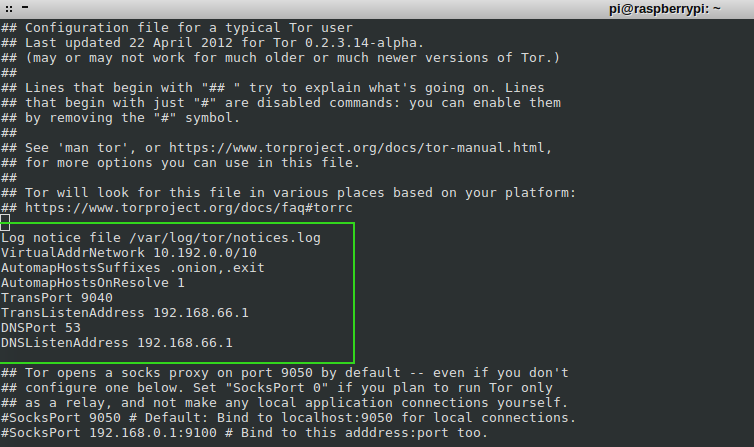
\includegraphics[scale=0.6]{images/torrc}
\caption{torrc Datei}
\end{figure}

Der Firewall muss jetzt noch beigebracht werden, dass jegliche Kommunikation vom WLAN-Netz über das Tor-Netzwerk weitergeleitet werden soll. \\
Dazu müssen folgende Befehle abgesetzt werden:

% FIXME: ssh chapter!

\begin{lstlisting}
iptables -F

iptables -t nat -F

iptables -t nat -A PREROUTING -i wlan0 -p tcp --dport 22 -j REDIRECT --to-ports 22

iptables -t nat -A PREROUTING -i wlan0 -p udp --dport 53 -j REDIRECT --to-ports 53

iptables -t nat -A PREROUTING -i wlan0 -p tcp --syn -j REDIRECT --to-ports 9040

iptables-save > /etc/iptables.ipv4.nat
\end{lstlisting}

In der \textit{torrc} Konfigurationsdatei wurde bei \textit{Log notice file} eine Datei angegeben, wo alle Logs hingeschrieben werden. Diese Datei muss nun erstellt und mit den entsprechenden Rechten versehen werden:

\begin{lstlisting}
touch /var/log/tor/notices.log
chown debian-tor /var/log/tor/notices.log
chmod 644 /var/log/tor/notices.log
\end{lstlisting}

Nun muss der Tor-Service noch neu gestartet werden, damit die vorgenommenen Einstellungen aktiv werden:

\begin{lstlisting}
service tor restart
\end{lstlisting}

Und um zu prüfen, ob Tor erfolgreich gestartet werden konnte, kann man folgenden Befehl ausführen:

\begin{lstlisting}
service tor status
\end{lstlisting}

Die Ausgabe sollte ähnlich dieser sein:

\begin{figure}[h]
\centering
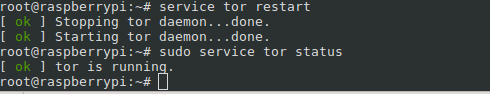
\includegraphics[scale=0.7]{images/tor_service}
\caption{Tor Service - Neustart und Status}
\end{figure}

Der Access Point und Tor sind an diesem Punkt fertig installiert und eingerichtet. Jetzt fehlt nur noch ein abschliessender Test, um sicherzustellen, dass alles so funktioniert, wie es soll.

\section{IP-Adresse verifizieren}
Mittels \url{ipchicken.com} kann die IP-Adresse ermittelt werden, mit der man sich im Internet bewegt. Diese wird einem normalerweise vom Provider zugeteilt und ändert sich eher selten. Mit einem funktionierenden Tor-Setup ändert sich dieses Verhalten jedoch. Da je Anfrage ins Internet drei verschiedene Tor-Server passiert, ändert sich die Absender-IP-Adresse des Paketes jedes Mal. Die angefragte Internetseite sieht somit nie die IP-Adresse, die einem vom Provider zugeteilt wurde, sondern immer die des zuletzt passierten Tor-Servers (Exit-Node). Um die korrekte Funktionsweise des Tor-Proxys zu verifizieren, muss man lediglich von einem Computer im normalen Netzt und einem Gerät, das mittels Tor-Proxy mit dem Internet verbunden is, \textit{ipchicken} aufrufen. Die IP-Adressen und auch die sonstigen angezeigten Informationen dürfen sich nicht decken. 
